%& --shell-escape dubble
%%%%%%%%%%%%%%%%%%%%%%%%%%%%%%%%%%%%%%%%%
% "Advances Towards Practical Implementations of Isogeny Based Signatures"
% Robert W. V. Gorrie - Master's Thesis Defense Presentaion
%
% McMaster University
% Department of Computing & Software
% November 2018
%
%%%%%%%%%%%%%%%%%%%%%%%%%%%%%%%%%%%%%%%%%

%----------------------------------------------------------------------------------------
%	PACKAGES AND THEMES
%----------------------------------------------------------------------------------------

\documentclass{beamer}

\mode<presentation> {
	\usetheme{Malmoe}                         % presentation layout theme
	\usecolortheme{dove}                      % presentation colour theme
	%\setbeamertemplate{footline}             % to remove the footer line in all slides uncomment this line
	\setbeamertemplate{footline}[page number] % replace the footer line in all slides with a simple slide count
	%\setbeamertemplate{navigation symbols}{} % remove the navigation symbols from the bottom of all slides
}

\usepackage{graphicx}                 % allows including images
\usepackage{booktabs}                 % allows the use of \toprule, \midrule and \bottomrule in tables
\usepackage{tikz}                     % include tikz for drawing figures
\usepackage{pgfplots}
\usepackage{amssymb, amsmath, amsthm}
\usepackage{xcolor,colortbl}          %for colouring in math mode
\usepackage{url}                      %for proper url entries
\usepackage{listings}                 %for writing c code
\usepackage{algorithm}
\usepackage{geometry}
\usepackage{tcolorbox}
\usepackage{xspace}

\usetikzlibrary{intersections,decorations.markings,matrix,calc,positioning,decorations.pathreplacing}

%----------------------------------------------------------------------------------------
%	STYLIZATIONS & OTHER COMMANDS
%----------------------------------------------------------------------------------------

\newcommand{\titlepageline}{%
	\tikz[remember picture,overlay] {%
		\draw[black] ([yshift=-4cm,xshift=\paperwidth/8]current page.north west)
				  -- ([yshift=-4cm,xshift=\paperwidth*7/8]current page.north west);}}

\newcommand{\topline}{%
	\tikz[remember picture,overlay] {%
		\draw[black] ([yshift=-1cm]current page.north west)
				  -- ([yshift=-1cm,xshift=\paperwidth]current page.north west);}}

\newcommand{\titleline}{%
	\tikz[remember picture,overlay] {%
		\draw[dashed] ([yshift=-2cm]current page.north west)
				  -- ([yshift=-2cm,xshift=\paperwidth]current page.north west);}}

\newcommand{\smallfont}{\fontsize{9}{7.2}\selectfont}

\newcommand{\mediumfont}{\fontsize{10}{7.2}\selectfont}

\newcommand{\largefont}{\fontsize{11}{7.2}\selectfont}

\newcommand{\plotcurve}[3][thick, every plot/.style={smooth}]{
  % plot curve y^2 = x^3 + a x + b in range [-3,3]^2
  % parameter 1 (optional): style options for curve (color, etc)
  % parameter 2: curve parameter a
  % parameter 3: curve parameter b
  \draw[->] (-4.2,0) -- (4.2,0) node[right] {$x$};         %x-axis
  \draw[->] (0,-4.2) -- (0,4.2) node[above] {$y$};         %y-axis
  \draw[->,>=latex,gray] (-3,0) -- (3,0);
  \draw[->,>=latex,gray] (0,-3) -- (0,3);
  \draw[name path=curve,black,thick] plot[id=curve#2#3, raw gnuplot] function {
    f(x,y) = y**2 - x**3 - #2*x - #3;
    set xrange [-3:3];
    set yrange [-3:3];
    set view 0,0;
    set isosample 500,500;
    set cont base;
    set cntrparam levels incre 0,0.1,0;
    unset surface;
    splot f(x,y);
  };
}

\newcommand{\mc}[2]{\multicolumn{#1}{c}{#2}}

\definecolor{Gray}{gray}{0.85}
\definecolor{LightCyan}{rgb}{0.88,1,1}
\definecolor{light-red}{RGB}{255,135,135}
\definecolor{light-green}{RGB}{135,255,135}
\definecolor{light-blue}{RGB}{135,135,255}
\newcolumntype{a}{>{\columncolor{Gray}}c}
\newcolumntype{b}{>{\columncolor{white}}c}

%----------------------------------------------------------------------------------------
%	TITLE PAGE
%----------------------------------------------------------------------------------------

\title[Practical PQ Signatures]{Advances Towards Practical Implementations of Isogeny Based Signatures} % The short title appears at the bottom of every slide, the full title is only on the title page

\author{Robert Gorrie} % Your name
\institute[McM] % Your institution as it will appear on the bottom of every slide, may be shorthand to save space
{
McMaster University --  Department of Computing \& Software \\ % Your institution for the title page
\medskip
\textit{gorrierw@mcmaster.ca} % Your email address
}
\date{\today} % Date, can be changed to a custom date

\begin{document}

\begin{frame}
\titlepage % Print the title page as the first slide
\topline
\titlepageline
\end{frame}

\begin{frame}
\frametitle{Overview} % Table of contents slide, comment this block out to remove it
\mediumfont
\topline
\titleline
\tableofcontents % Throughout your presentation, if you choose to use \section{} and \subsection{} commands, these will automatically be printed on this slide as an overview of your presentation
\end{frame}

%----------------------------------------------------------------------------------------
%	PRESENTATION SLIDES
%----------------------------------------------------------------------------------------

%------------------------------------------------
\section{Introduction \& Background}
%------------------------------------------------

\subsection{Post-quantum Cryptography \& Motivation}

\begin{frame}
\frametitle{Public-key Cryptography}
\topline
\titleline
There are five rudimentary concerns of information security:
\begin{itemize}
\item \textit{Confidentiality}: information must be kept private from unauthorized individuals
\item \textit{Integrity}: information must not be altered by unauthorized individuals
\item \textit{Availability}: information must be available for authorized individuals
\item \textit{Authenticity}: information must have a verifiable source
\item \textit{Non-repudiation}: the source of information must be publicly verifiable
\end{itemize}
\end{frame}

%------------------------------------------------

\begin{frame}
\frametitle{Public-key Cryptography}
\topline
\titleline
The goal of cryptography is to define mathematically precise means of ensuring these information security goals.\\
\vspace{20px}

Cryptographic protocols can be either \textit{private-key} or \textit{public-key} systems.\\
\vspace{20px}

Public-key systems require that every party takes ownership of both a public key ($pk$), the value of which is known by everyone on the network, and a private key ($sk$), known only to the owner.
\vspace{20px}
\end{frame}

%------------------------------------------------

\begin{frame}
\frametitle{Quantum Cryptanalysis}
\topline
\titleline
Efficient large-scale quantum computing $\rightarrow$ breaking most modern public-key cryptosystems.\\
\vspace{25px}

This has lead to the development of the field known as post-quantum cryptography -- the aim of which is to develop cryptosystems resistant to quantum cryptanalysis.
\end{frame}

%------------------------------------------------

\begin{frame}
\frametitle{Post-quantum Cryptography}
\topline
\titleline
Common approaches to post-quantum cryptography include
\begin{itemize}
\item Lattice-based cryptography
\item Hash-based cryptography
\item Multivariate-based cryptography
\item Code-based cryptography
\item Isogeny-based cryptography
\end{itemize}
\end{frame}

%------------------------------------------------

\begin{frame}
\frametitle{Post-quantum Cryptography}
\topline
\titleline
\begin{figure}[!h,scale=0.25]
  \begin{center}
    \begin{tabular}{ l | r | r | r }
      \hline
      \mc{1}{}  & \mc{1}{Key Gen} & \mc{1}{Sign} & \mc{1}{Verify}\\
      \hline
      \rowcolor{Gray}
      SIDH & 84,499,270 & 4,950,023,141.65 & 3,466,703,991.09 \\
      Sphincs & 17,535,886.94 & 653,013,784 & 27,732,049 \\
      qTESLA & 1,059,388 & 460,592 & 66,491 \\
      Picnic & 13,272 & 9,560,749 & 6,701,701 \\
      \rowcolor{light-red}
      RSA & 12,800,000 & 1,113,600 & 32400 \\
      \rowcolor{light-red}
      ECDSA & 1,470,000 & 128,928 & 140,869 \\
      \hline
    \end{tabular}
  \end{center}
\end{figure}
\end{frame}

%------------------------------------------------

\subsection{Elliptic Curves \& Isogenies}

\begin{frame}
\frametitle{Elliptic Curves as a Group}
\topline
\titleline
Elliptic curves are a class of algebraic curves satisfying

\begin{columns}[c]
\column{.45\textwidth}
  $$
  E: y^2 = x^3 + ax + b.
  $$
  \vspace{5px}
  We can define a group composed of all the points $P = (x, y)$ satisfying $E$.

\column{.45\textwidth}
  \begin{figure}[!h]
    \begin{tikzpicture}[scale=0.5]
      \plotcurve{-2}{2}
    \end{tikzpicture}
  \end{figure}
\end{columns}
\end{frame}

%------------------------------------------------

\begin{frame}
\frametitle{Elliptic Curves as a Group}
\topline
\titleline

\begin{figure}[!h]
\begin{tikzpicture}[scale=0.7]
  \plotcurve{-2}{2}
  \draw [] (-1.73,0.531) -- (1.564,1.642);
  \draw [dashed] (1.564,1.642) -- (1.564,-1.642);
  \draw[fill] (-1.73,0.531) circle (0.1) node[right] {$P$};
  \draw[fill] (0.28,1.209) circle (0.1) node[right] {$Q$};
  \draw[fill] (1.564,1.642) circle (0.1) node[right] {$R$};
  \draw[fill] (1.564,-1.642) circle (0.1) node[right] {$R' = P+Q$};
\end{tikzpicture}
\end{figure}
\end{frame}

%------------------------------------------------

\begin{frame}
\frametitle{Isogenies}
\topline
\titleline
Isogenies are maps that take a point on one elliptic curve to a point on another.
For an isogeny $\phi$ mapping from $E_1$ to $E_2$, we can write
$$
\phi: E_1 \rightarrow E_2
$$
These maps have the following two properties
\begin{itemize}
  \item $\phi(\mathcal{O}) = \mathcal{O}$
  \item $\phi(P^{-1}) = (\phi(P)^{-1})$
\end{itemize}
\end{frame}

%------------------------------------------------

\subsection{Supersingular Isogeny Diffie-Hellman}

\begin{frame}
\frametitle{Key Exchange Protocols}
\topline
\titleline
Key exchange protocols are cryptographic schemes used to establish a shared secret between two party members\\

These can be defined by a tuple of algorithms $\Pi_{kex} = (\textbf{KeyGen}, \textbf{SecAgr})$.

\end{frame}

%------------------------------------------------

\begin{frame}
\frametitle{Key Exchange Protocols}
\topline
\titleline
\begin{center}
  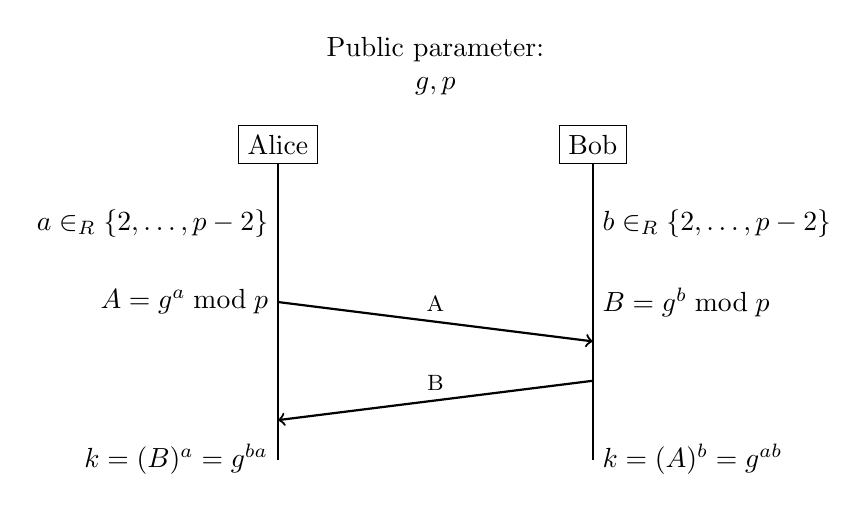
\begin{tikzpicture}
    % Public parameter:
    \node[draw=none,fill=none,align=center] (public) at (0,1) {Public parameter:\\$g, p$};

    % Alice
    \node[draw] (Alice) at (-2,0) {Alice};
    \draw[thick] (Alice) -- ++(0, -4);

    % Calculations of Alice
    \node[draw=none,fill=none,anchor=east] (asecret) at ($(Alice) + (0,-1)$) {$a \in_{R} \{2,\dots,p-2\}$};
    \node[draw=none,fill=none,anchor=east] (Apublic) at ($(Alice) + (0,-2)$) {$A = g^{a} \bmod{p}$};
    \node[draw=none,fill=none,anchor=east] (akey) at ($(Alice) + (0,-4)$) {$k = (B)^{a} = g^{ba}$};

    % Bob
    \node[draw] (Bob) at (2,0) {Bob};
    \draw[thick] (Bob) -- ++(0, -4);

    % Calculations of Bob
    \node[draw=none,fill=none,anchor=west] (bsecret) at ($(Bob) + (0,-1)$) {$b \in_{R} \{2,\dots,p-2\}$};
    \node[draw=none,fill=none,anchor=west] (Bpublic) at ($(Bob) + (0,-2)$) {$B = g^{b} \bmod{p}$};
    \node[draw=none,fill=none,anchor=west] (bkey) at ($(Bob) + (0,-4)$) {$k = (A)^{b} = g^{ab}$};

    % Messages
    \draw[->,thick] ($(Alice)+(0,-2)$) -- ($(Bob)+(0,-2.5)$) node [pos=0.5,above,font=\footnotesize] {A};
    \draw[->,thick] ($(Bob)+(0,-3)$) -- ($(Alice)+(0,-3.5)$) node [pos=0.5,above,font=\footnotesize] {B};
  \end{tikzpicture}
\end{center}
\end{frame}

%------------------------------------------------


\begin{frame}
\frametitle{Supersingular Isogeny Diffie-Hellman}
\topline
\titleline

\end{frame}

%------------------------------------------------

\subsection{Isogeny-based Signatures}

\begin{frame}
\frametitle{Interactive Identification Schemes}
\topline
\titleline
\begin{theorem}[Mass--energy equivalence]
$E = mc^2$
\end{theorem}
\end{frame}

%------------------------------------------------

\begin{frame}
\frametitle{Signature Schemes}
\topline
\titleline
\begin{theorem}[Mass--energy equivalence]
$E = mc^2$
\end{theorem}
\end{frame}

%------------------------------------------------

\begin{frame}
\frametitle{Fiat-Shamir Transform}
\topline
\titleline
\begin{theorem}[Mass--energy equivalence]
$E = mc^2$
\end{theorem}
\end{frame}

%------------------------------------------------

\begin{frame}
\frametitle{Yoo Signatures}
\topline
\titleline
\begin{theorem}[Mass--energy equivalence]
$E = mc^2$
\end{theorem}
\end{frame}


%------------------------------------------------
\section{Batching Field Element Inversions}
%------------------------------------------------

\subsection{Batching Partial Inversions}

\begin{frame}
\frametitle{Table}
\topline
\titleline
\begin{table}
\begin{tabular}{l l l}
\toprule
\textbf{Treatments} & \textbf{Response 1} & \textbf{Response 2}\\
\midrule
Treatment 1 & 0.0003262 & 0.562 \\
Treatment 2 & 0.0015681 & 0.910 \\
Treatment 3 & 0.0009271 & 0.296 \\
\bottomrule
\end{tabular}
\caption{Table caption}
\end{table}
\end{frame}

%------------------------------------------------

\subsection{Implementing Batching in SIDH 2.0}

\begin{frame}
\frametitle{Signature Schemes}
\topline
\titleline
\begin{theorem}[Mass--energy equivalence]
$E = mc^2$
\end{theorem}
\end{frame}

%------------------------------------------------

\subsection{Performance of Inversion Batching}

\begin{frame}[fragile] % Need to use the fragile option when verbatim is used in the slide
\frametitle{Verbatim}
\topline
\titleline
\begin{example}[Theorem Slide Code]
\begin{verbatim}
\begin{frame}
\frametitle{Theorem}
\begin{theorem}[Mass--energy equivalence]
$E = mc^2$
\end{theorem}
\end{frame}\end{verbatim}
\end{example}
\end{frame}

%------------------------------------------------
\section{Compressing Isogeny-based Signatures}
%------------------------------------------------

\subsection{SIDH Public Key Compression}

\begin{frame}
\frametitle{Figure}
\topline
\titleline
Uncomment the code on this slide to include your own image from the same directory as the template .TeX file.
%\begin{figure}
%\includegraphics[width=0.8\linewidth]{test}
%\end{figure}
\end{frame}

%------------------------------------------------

\subsection{Implementing in SIDH 2.0}

\begin{frame}[fragile] % Need to use the fragile option when verbatim is used in the slide
\frametitle{Citation}
\topline
\titleline
An example of the \verb|\cite| command to cite within the presentation:\\~

This statement requires citation \cite{p1}.
\end{frame}

%------------------------------------------------

\subsection{Advantage and Cost of Compressions}

\begin{frame}[fragile] % Need to use the fragile option when verbatim is used in the slide
\frametitle{Citation}
\topline
\titleline
An example of the \verb|\cite| command to cite within the presentation:\\~

This statement requires citation \cite{p1}.
\end{frame}

%------------------------------------------------
\section{Results}
%------------------------------------------------

\subsection{Performance Measurements}

\begin{frame}
\Huge{\centerline{Questions?}}
\end{frame}

%------------------------------------------------

\begin{frame}
\frametitle{References}
\topline
\titleline
\footnotesize{
\begin{thebibliography}{99} % Beamer does not support BibTeX so references must be inserted manually as below
\bibitem[Smith, 2012]{p1} John Smith (2012)
\newblock Title of the publication
\newblock \emph{Journal Name} 12(3), 45 -- 678
\end{thebibliography}
}
\end{frame}

%----------------------------------------------------------------------------------------

\end{document}
